\documentclass[11pt, a4paper]{article}
\usepackage[utf8]{inputenc}
\usepackage[T1]{fontenc}                 % Umlaute und co
\usepackage[ngerman]{babel}              % Deutsche Trennung von Wörtern
\usepackage{graphicx}                    % Für includegraphics
\usepackage{enumitem}                    % Abstände zwischen Listen und Aufzählungen
\usepackage{tikz}                        % Zeichnen von Diagrammen
\usepackage{caption}                     % Beschriftung von Abbildungen
\usepackage{amsmath}                     % Mathematische Gleichungen besser formatieren
\usepackage{pgfplots}                    % Zeichnen von Daten
\usepackage{pgfplotstable}

\usetikzlibrary{arrows} 

\tikzstyle{arrow} = [thick,->,>=stealth]
\tikzstyle{box}=[draw, minimum size=2em]

\begin{document}

\begin{titlepage}
    \title{Die gedanken eines Mathematikers über die COVID-19}
    \author{Janos Sarközi}
    \maketitle
\end{titlepage}

\section{Einführung}

Die Ausbreitung eines Viruses kann durch die Modellierung eines dynamischen System erreicht
werden. Dafür wird die Befölkerung in vier Gruppen unterteilt.

\begin{itemize}[itemsep=0pt]
    \item Anfällig
    \item Krank
    \item Immun
    \item Tot
\end{itemize}

Zwischen diesen Personen wird durch die Krankheit ein Austausch statt finden. Dies kann
in ein Diagramm zusammengefasst werden. Dabei kürzen wir die vier Zustände Anfällig = A,
Krank = K, Immun = I und Tot = T ab.

\begin{figure}[h]
\centering
\begin{tikzpicture}
    \node (s) [box]                                  {A};
    \node (i) [box, node distance=2.2cm, right of=s] {K};
    \node (r) [box, node distance=2.2cm, right of=i] {I};
    \node (d) [box, node distance=2.0cm, below of=i] {T};
    \draw [arrow] (s) -- (i);
    \draw [arrow] (i) -- (r);
    \draw [arrow] (i) -- (d);
\end{tikzpicture}
\caption{Zustandsänderung der Befölkerung}
\label{fig:sir}
\end{figure}

In Abbildung \ref{fig:sir} ist folgendes zu sehen. Aus anfälligen Personen können durch den Virus Kranke personen werden. Die kranken Personen können gesund werden und eine Immunität daruch
erlangen oder Sie sterben. Es stellt sich noch dir Frage, ob immune Personen doch nicht die
Immunität haben wie gedacht und wieder anfällig werden können? Einfachheits halber, sollen
die immune Personen immun bleiben. In der Abbildung 1 soll auch ein einfaches Modell
betrachtet werden. Es gibt natürlich auch kompliziertere Modelle, aber sehen wir mal an,
wie weit wir mit diesem Modell kommen.

\newpage
\section{Etwas Mathematik}
Erweitert man die Abbildung 1 wie folgt:
\begin{figure}[h]
\centering
\begin{tikzpicture}
    \node (s) [box]                                  {A};
    \node (i) [box, node distance=2.2cm, right of=s] {K};
    \node (r) [box, node distance=2.2cm, right of=i] {I};
    \node (d) [box, node distance=2.0cm, below of=i] {T};
    \draw [arrow] (s) -- (i) node[midway, above=2pt, fill=none] {$\beta$AK};
    \draw [arrow] (i) -- (r) node[midway, above=2pt, fill=none] {$\gamma$K};
    \draw [arrow] (i) -- (d) node[midway, right=2pt, fill=none] {$\delta$K};
\end{tikzpicture}
\caption{Dynamisches Modell}
\label{fig:dynModel}
\end{figure}

Dann kann ein Differentialgleichungssystem aufgeschrieben werden. Es beschreibt die
Änderung der Zustände der Personen.

\begin{equation}
    \begin{aligned}
        \frac{dA}{dt} &= -\beta AK                      \\[5pt]
        \frac{dK}{dt} &= \beta AK - \gamma K - \delta K \\[5pt]
        \frac{dI}{dt} &= \gamma K                       \\[5pt]
        \frac{dT}{dt} &= \delta K                       \\[10pt]
    \end{aligned}
\end{equation}

Diese Gleichungen können leicht aus der Abbildung \ref{fig:dynModel} aufgeschrieben werden.
Die erste Gleichungen ist aus dem Pfeil von A nach K herzuleiten. Der Pfeil zeigt im
gewissen sinne die Wanderung von Personen von einem zustand in das nächste. Da der Pfeil
aus A kommt, wird die Funktion $\beta$AK mit einem minus bewertet. Für den Kasten K kommen
drei Pfeile in Frage. Ein Pfeil trifft K und zwie Pfeile verlassen K. Damit sind die letzen
beiden Gleichungen mit I und T klar.

\section{Lösen der Gleichungen}

Für das Lösen des Gleichungssystems kramt man sich aus dem Internet etwas raus. Ich habe
mich für  Jupyther Notebook entschieden. Das Ergebnis sieht dann so aus:

% \begin{figure}
%     \centering
%     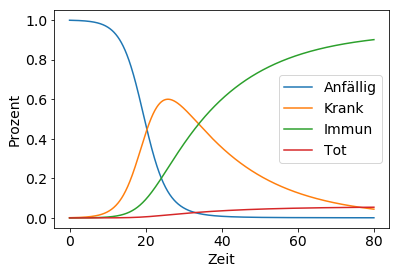
\includegraphics{images/Download.png}
%     \caption{Meine Grafik}
%     \label{fig:meine-grafik}
% \end{figure}
% 
\begin{tikzpicture}
    \begin{axis}[xlabel=Q Series, ylabel=P Values]
        \addplot table [y=P, x=$Q_A$] {data/data.dat};
        \addlegendentry{$Q_A$ series}
        \addplot table [y=P, x=$Q_B$] {data/data.dat};
        \addlegendentry{$Q_B$ series}
        \addplot table [y=P, x=$Q_D$] {data/data.dat};
        \addlegendentry{$Q_D$ series}
    \end{axis}
\end{tikzpicture}

\begin{tikzpicture}
    \begin{axis}[xlabel=Q Series, ylabel=P Values]
        \addplot table [x=Name, y=Age, col sep=comma] {data/asdf.csv};
        \addlegendentry{$Q_A$ series}
        \addplot table [x=Name, y=Bla, col sep=comma] {data/asdf.csv};
        \addlegendentry{$Q_B$ series}
    \end{axis}
\end{tikzpicture}

\end{document}
